% -*- root: main.tex -*-
% !TEX root = main.tex
The main \emph{goal} of our study is to better understand what happens to \SATD once it is introduced into software projects. To do so, our first step is to quantify how much of \SATD comments get removed (RQ1). Next, we analyze who removes \SATD, i.e., if the same developer that introduced the debt is also most likely to remove it (RQ2). Then, we investigate how long the \SATD remains in the project (RQ3). Finally, we conduct a survey with 14 developers to understand why \SATD is introduced and removed (RQ4). For each question, we describe the motivation behind it, the approach chosen to address it, and the results obtained.

\begin{table}[!t]
	\begin{center}
		\caption{\textsc{Removed \SATD per project.}}
		\label{tbl:removed_self_admitted_technical_debt_per_project}
		\begin{tabular}{l|rrrr}
			\toprule
			\textbf{\thead{Project}} & \textbf{\thead{\# Identified}} & \textbf{\thead{\# Removed}} & \textbf{\thead{\% Removed}} &  \textbf{\thead{\% Remaining}}  \\ 
			\midrule
			\textbf{Camel }  &  4,331  & 3,926  & 90.6  & 9.4\\
			\textbf{Gerrit}  &  271    & 208    & 76.7 & 23.3 \\
			\textbf{Hadoop}  &  1,164  & 472    & 40.5 & 59.5 \\  
			\textbf{Log4j }  &  135    & 118    & 87.4 & 12.6\\ 
			\textbf{Tomcat}  &  1,317  & 1,009  & 76.6 & 23.4\\   
			\midrule
			\textbf{Average} & -       & -      & 74.4 & 25.6\\
			\textbf{Median} & -       & -      & 76.7 & 23.3\\
			\bottomrule
		\end{tabular}
	\end{center}    
\end{table}


\subsection*{\rqi}
\subsubsection*{Motivation} Previous work showed that technical debt is widespread, unavoidable, and has arguably some negative impact on software projects~\cite{Lim2012Software}. Therefore, a priori we expect that removing technical debt is a concern for developers. To understand how developers deal with  technical debt we must first quantify how much debt is removed. 


\subsubsection*{Approach} To answer this question we automatically identify \SATD from the five analyzed projects. As described in Section~\ref{sub:checkout_all_versions_of_files}, we stored all versions of all source code files. Then, for each analyzed \SATD comment we take the oldest file version available in which the debt was found and incrementally search for matches in future versions of the file. The first time that the analyzed \SATD comment(s) appears in a file, indicates the exact file version that the \SATD comment was introduced. To analyze if the introduced \SATD comment was later removed, we search for the same comment in the remaining file versions. When the comment is no longer found, we mark that version of the file as the removal version. In certain cases, a \SATD comment is found in one version only (i.e., the version that it is introduced in). Such cases indicate a scenario where the \SATD was introduced and removed immediately after. 



\subsubsection*{Results} Table \ref{tbl:removed_self_admitted_technical_debt_per_project} presents the identified and removed \SATD comments. We find that the majority (\textit{i.e.,} on average 74.4\%, median 76.7\%) of the identified \SATD comments were removed. We measure the average on a per project basis, \textit{i.e.,} the total from each project is taken and the average/median over the five projects are provided. For example, we find 271 unique instances of \SATD comments when analyzing the Gerrit project. 76.7\% (\textit{i.e.,} 208) of these \SATD comments were removed during the evolution of the project. Camel had the highest \SATD comments removal percentage (\textit{i.e.,} 90.6), whereas Hadoop had the lowest removal percentage reaching 40.5\%. 

Our findings indicate that developers tend to be aware and do care about \SATD. This finding corroborates with the survey findings of Ernst \emph{et al.}~\cite{Ernst2015FSE}. Also, these results match those observed in earlier studies reported by Potdar and Shihab~\cite{Potdar2014ICSME} and Bavota and Russo~\cite{Bavota2016MSR}.






\conclusion{The majority of \SATD comments are removed over time. In our five case study projects, between 40.5--90.6\% (median 76.7\%) of the identified \SATD is removed.}
 

\subsection*{\rqii}

\subsubsection*{Motivation} As opposed to the technical debt in general, \emph{self-admitted} technical debt stands for technical debt \emph{confessed} by the developers themselves. This intuition leads us to believe that it would be natural that the developers who expressed concern about the code would be also the ones who fix it in the future. However, it is unknown whether this is the case. It makes intuitive sense that self-removal of \SATD is easier, since the developers know about the reason for the \SATD introduction and possibly how to address it. The findings of this question have implications on the way that developers/manager/projects need to manage \SATD. For example, if it is found that \SATD is mostly addressed by others, then projects need to pay special attend to how this technical debt (and the areas of the code that it exists in) is documented. If on the other hand, it is indeed mostly self-removed, then the problem is less troubling.



\subsubsection*{Approach} To answer this question we analyzed the authors of the changes (\textit{i.e.,} commits from the source code repository) that introduced or removed \SATD comments. In order to do that, we first determine the commit in which a \SATD comment was added, then we check the further file versions to determine if there is any commit that removed the \SATD comment. Finally, we compare the authors of the commits to see if they are the same or not. 

We take into consideration two attributes of the change when comparing authors---the author name and email address. This is a necessary heuristic to mitigate the risk of misclassifying authors that change their names in the source code repository during the evolution of the project.  




\subsubsection*{Results} Table~\ref{tbl:self_removed_technical_debt_vs_non_self_removed_technical_debt_per_project} shows that in most cases, the majority of \SATD is removed by the same author who introduced it, referred to as ``self-removed technical debt''. On average, 54.4\% of all removals are self-removed and in four of the five projects, self-removal accounts for more than 50\%.  This finding agrees with Bavota and Russo's study, which found that \SATD is self-removed in 63\% of the cases in their dataset. Once again, we measure the average on a per project basis, \emph{i.e.}, the total from each project is taken and the average over the five projects in provided. The project with highest percentage of self-removed technical debt was Gerrit with 71.6\%, and the lowest percentage---Hadoop with 24.6\%. 

Hadoop tends to be an outlier in terms of self-removed \SATD, however, it is worth mentioning that Hadoop had the least amount of removals overall (only 40.5\% of the \SATD is ever removed). There are many possible reasons for the low removal rates, \emph{e.g.}, high developer churn or lack of process to deal with technical debt. Although we shed some light on the potential reasons for the removal of \SATD later in RQ4, we believe that determining the exact reasons for \SATD removal warrant a study on its own.


\conclusion{The majority of \SATD is self-removed. On average 54.4\% of \SATD is self-removed and on median 61.0\% is self-removed.}


\begin{table}[!t]
	\begin{center}
		\caption{\textsc{Self-removed technical debt per project.}}
		\label{tbl:self_removed_technical_debt_vs_non_self_removed_technical_debt_per_project}
		\begin{tabular}{l|rrr}% | c c}
			\toprule
			\textbf{\thead{Project}} & \textbf{\thead{\# Removed}} & \textbf{\thead{\# Self-removed}} & \textbf{\thead{\% Self-removed} }\\
			\midrule
			\textbf{Camel }   & 3,926 & 2,652 & 67.5 \\%&  1,274 & 32.5 \\  
			\textbf{Gerrit}   & 208   &  149  & 71.6 \\%&    59  & 28.4 \\  
			\textbf{Hadoop}   & 472   &  116  & 24.6 \\%&   356  & 75.4 \\  
			\textbf{Log4j }   & 118   &   72  & 61.0 \\%&    46  & 39.0 \\  
			\textbf{Tomcat}   & 1,009 &  578  & 57.3 \\%&   431  & 42.7 \\  
			\midrule
			\textbf{Average} & -      & -     & 54.4\\% &    -   & 43.6 \\
			\textbf{Median}  & -      & -     & 61.0 \\%&    -   & 39.0 \\
			\bottomrule
		\end{tabular}
	\end{center}    
\end{table}



\subsection*{\rqiii}


\subsubsection*{Motivation} From RQs 1 and 2, we know that the majority of \SATD is removed and most of the time it is removed by the same developer who introduced it. Next, we would like to know how long \SATD lives in a project before it is actually removed. Answering this question helps us to understand for how long it is normal to have \SATD comments in the projects. In addition, once we quantify the number of self-removed technical debt and the number of non-self-removed technical debt comments, we would like to understand if these two categories of removal have differences between them. For example, since we know that the majority of \SATD is self-removed, is it the case that it is removed faster? since our intuition is that it would be easier to be addressed. 

\subsubsection*{Approach} To determine the amount of time that \SATD lives in a project, we use the time difference between the commit that introduces and removes the \SATD comment. The steps to identify the \SATD introducing and removing commits are the same as we outlined in RQs 1 and 2. We measure the average and median time for \SATD to be removed. It is important to note that the timezone is irrelevant in this analysis since we normalize the data used in our survival plots by calculating the delta between insertion and removal of SATD from each project separately (i.e., on their own repositories timezone).

Additionally, we generate survival plots for the removal of \SATD to determine how likely the technical debt will live in a project. Survival plots show the (general) trend times for a given event to occur. In our case, the survival plots show the  percentage of self-admitted technical debt that survives in a project overtime. Finally, we distinguish between self- and non-self-removed technical debt and compare the removal time of each. We compare the two distributions (\emph{i.e.}, self- and non-self-removal) using a Mann-Whitney test~\cite{mann1947test} to determine if the difference is statistically significant at the customary level of 0.05.




\begin{figure}[t]
	\centering
	\includegraphics[width=\columnwidth]{figures/test/distribution_.pdf}
	\caption{The distribution of times of all the removed \SATD comments.}
	\label{fig:removed_all_std_comments}
\end{figure}




\begin{figure*}[t]
	\centering
	
	\begin{subfigure}[b]{0.31\textwidth}
		\includegraphics[width=\textwidth]{figures/Survival/camel.pdf}
	\end{subfigure}
	~
	~
	\begin{subfigure}[b]{0.31\textwidth}
		\includegraphics[width=\textwidth]{figures/Survival/gerrit.pdf}
	\end{subfigure}
	~
	~
	\begin{subfigure}[b]{0.31\textwidth}
		\includegraphics[width=\textwidth]{figures/Survival/hadoop.pdf}
	\end{subfigure}
	
	
	\begin{subfigure}[b]{0.31\textwidth}
		\includegraphics[width=\textwidth]{figures/Survival/log4j.pdf}
	\end{subfigure}
	~
	~
	\begin{subfigure}[b]{0.31\textwidth}
		\includegraphics[width=\textwidth]{figures/Survival/tomcat.pdf}
	\end{subfigure}
	\caption{Survival plots show the probability of the removal of \SATD comment for all studied projects.}
	\label{fig:survival_plots}
\end{figure*}


\begin{table}[t]
	\begin{center}
		\caption{\textsc{Self-removal vs non-self-removal: Mann-Whitney Test ($p$-value) and Cliff's Delta ($d$)}.}
		\label{tbl:statistic}
		\begin{tabular}{l| rrr}
			\toprule
			\textbf{\thead{Project}} & \textbf{\thead{$p$-value}}&~~~ & \textbf{\thead{$d$}}\\ 
			\midrule
			\textbf{Camel }   &  0.000125& ~~~ &  $-$0.075(medium)\\  
			\textbf{Gerrit}   &  3.581e-14& ~~~ &  $-$0.671(large)\\  
			\textbf{Hadoop}   &  $<$ 2.2e-16& ~~~ &  $-$0.531(large)\\  
			\textbf{Log4j}   &  2.345e-06 & ~~~ &  $-$0.517(large)\\  
			\textbf{Tomcat}   &  $<$ 2.2e-16  & ~~~ &  $-$0.820(large)\\  
			\bottomrule
		\end{tabular}
	\end{center} 
	\vspace{-0.1in}   
\end{table}




We estimated the magnitude of the difference between self-removed technical debt and non-self-removed technical debt using the Cliff's Delta (or $d$)~\cite{grissom2005effect}, a non-parametric effect size measure for ordinal data. We consider the effect size values: small for $d$ $<$ 0.33 (positive as well as negative values), medium for 0.33  $\leq d<$ 0.474 and large for $d \geq$ 0.474.

\subsubsection*{Results} Figure~\ref{fig:removed_all_std_comments} shows the distribution, the mean and median times for removal of the \SATD. The distribution of \SATD removal is skewed, as indicated by plots and the difference in the mean and median removal times. In general, the time that \SATD stays in a project  varies from one project to another: medians range between 18.2--172.8 days and averages---82--613.2 days. One clear finding however, is that in Camel and Gerrit, \SATD is removed faster than in Hadoop, Log4j and Tomcat.

Figure~\ref{fig:survival_plots} shows the survival plots of \SATD for the five studied projects. Survival plot is a technique originating from the medical domain indicating the probability of a patient to survive at least for $x$ days. To estimate this probability one would ideally like to 
have complete information about the death time of all patients. Such an assumption is, however, usually not realistic as some patients might still be alive at the end of the observations, \emph{i.e.}, the data is right-censored. Kaplan and Meier~\cite{kaplan1958nonparametric} have proposed a technique to estimate the survival in presence of right-censored data. As we have seen in Table~\ref{tbl:removed_self_admitted_technical_debt_per_project} some \SATD comments remained at the end of the observations, \emph{i.e.}, our data is also right-censored, in Figure~\ref{fig:survival_plots} we present the Kaplan-Meier estimators. The use of Kaplan-Meier estimators is common in software evolution applications of survival analysis~\cite{samoladas2010survival,goeminne2015towards,Lin:et:al}.

Inspecting Figure~\ref{fig:survival_plots} we observe that for all projects, there is a steep decline in the first few hundred days, suggesting that in all projects an important share of \SATD is rapidly removed. Projects do differ in how steep the drop is and where it flattens out. For example, for Camel  there is a steep drop in \SATD after around 48 days and a long tail after that. This means that in Camel, the likelihood of \SATD surviving (\emph{i.e.}, existing in the project after introduction) drops sharply after 48 days, and after that time, the chance of surviving is less than 20\%, as indicated by the survival function. Another extreme case is Hadoop, where the chance of \SATD surviving for more than 1,150 days is close to 57.8\%; the percentage
of the \SATD comments remaining at the end of the observations reported in Table~\ref{tbl:removed_self_admitted_technical_debt_per_project}. 




We also compare the time that self-removed and non-self-removed \SATD exists in the project before it gets removed. We find that self-removed technical debt gets removed faster than non-self-removed technical debt. Figure~\ref{fig:removal_self_vs_nonself} shows that, on median for all projects, self-removed technical debt is removed earlier than non-self-removed technical debt. Our finding confirms our intuition, however, the exact reasons (e.g., is it because the remover is more familiar with the debt) as to why self-removals take less time warrant a study on its own. Table~\ref{tbl:statistic} shows the result of  Mann-Whitney test and Cliff's Delta ($d$), which is a measure of effect size. We observe that for all the studied projects the difference between self-removed and non-self-removed technical debt is statistically different. The effect size, for all the projects is large except for Camel, where the effect size is medium.

\conclusion{The amount of time \SATD remains in a project before removal varies from one project to another and ranges between 18.2--172.8 days on median and 82--613.2 days on average. Moreover, self-removed technical debt is removed faster than non-self-removed technical debt.}




\begin{figure*}[t]
	\centering
	\begin{subfigure}[b]{0.195\textwidth}
		\includegraphics[width=\textwidth]{figures/test/Camel.pdf}
		\label{fig:removal_comparison_camel}
	\end{subfigure}
	\begin{subfigure}[b]{0.193\textwidth}
		\includegraphics[width=\textwidth]{figures/test/Gerrit.pdf}
		\label{fig:removal_comparison_gerrit} 
	\end{subfigure}
	\begin{subfigure}[b]{0.195\textwidth}
		\includegraphics[width=\textwidth]{figures/test/Hadoop.pdf}
		\label{fig:removal_comparison_hadoop} 
	\end{subfigure}
	\begin{subfigure}[b]{0.191\textwidth}
		\includegraphics[width=\textwidth]{figures/test/Log4j.pdf}
		\label{fig:removal_comparison_log4j}
	\end{subfigure}
	\begin{subfigure}[b]{0.195\textwidth}
		\includegraphics[width=\textwidth]{figures/test/Tomcat.pdf}
		\label{fig:removal_comparison_tomcat} 
	\end{subfigure}
	\begin{subfigure}[b]{0.30\textwidth}
		\includegraphics[width=\textwidth]{figures/test/legend_.pdf}
	\end{subfigure}
	\caption{Self-Removal vs Non Self-Removal for all studied projects.}
	\label{fig:removal_self_vs_nonself}
\end{figure*}










\subsection*{\rqiv}


\subsubsection*{Motivation} 
Thus far, our analysis has been quantitative in nature. To triangulate our findings and better understand our findings, we perform complementary qualitative analysis to understand the experiences and motives of developers who introduce and remove \SATD.



 
\subsubsection*{Approach} 
To understand the activities that lead to the introduction and removal of \SATD, we designed an online survey. 
While participants have been purposefully recruited, we did not store any identifying information  about the individual respondents\textbf{AS: 1) please provide the link to the survey form; 2) are we sure that developers couldn't be identified based on the project/addd or removed SATD? Can we report the number of such developers per project? 3) any other ethical risks?}.

The survey included three main sections: 1)  questions regarding the participant's role and development tasks and experience in the project, 2) three Likert-scale questions about the frequency of developers encountering, adding, and addressing self-admitted technical debt, and 3) two open ended questions asking why developers add or remove \SATD. 

To identify the target population, we collected the names and email addresses of all developers who added or removed self-admitted technical debt in the five studied projects and an additional two projects from the training dataset, namely Apache Ant and Jmeter. We chose these two additional projects to increase the potential number of respondents and to avoid including all of the training dataset projects to not overwhelm developers with requests for surveys.

In total, we found 250 unique developers from the studied projects and we successfully sent the survey to 188 of them.  We received 14 responses, \emph{i.e.}, the response rate is 7.4\%. Although this is lower than the response rate reported in software engineering surveys \cite{Punter2003}, the area of technical debt is difficult to discuss, especially since some developers may feel they will be negatively perceived. Half of the respondents were from the five studied projects and the other half were from the Apache Ant and Jmeter projects. For the open-ended questions, we manually analyzed the free-text answers and identified six main reasons why developers add self-admitted technical debt and five main reasons for removing self-admitted technical debt. Of the 14 respondents, eight identified themselves as core developers, and six as contributors to the projects. Five of the 14 respondents work on fixing bugs, and five work on implementing new features. Only one respondent has the task of code reviewer. Another three respondents indicted having different tasks (\emph{e.g.}, project user). Twelve respondents have more than five years of experience and only two respondents have less than three years of experience.




\subsubsection*{Results} 
Figure~\ref{fig:encouner_add_address} shows the results of the Likert-scale questions about how often developers encounter, add, address self-admitted technical debt. Developers mostly agreed that they encounter source code comments indicating self-admitted technical debt. 




All respondents report that they encounter \SATD comments at least as often as add them or address them. Interestingly enough six respondents indicate that they add \SATD comments more often than address them, while only three indicate the opposite, i.e., that they address \SATD comments more often then add them.


 
 \begin{figure}[t]
 	\centering
 	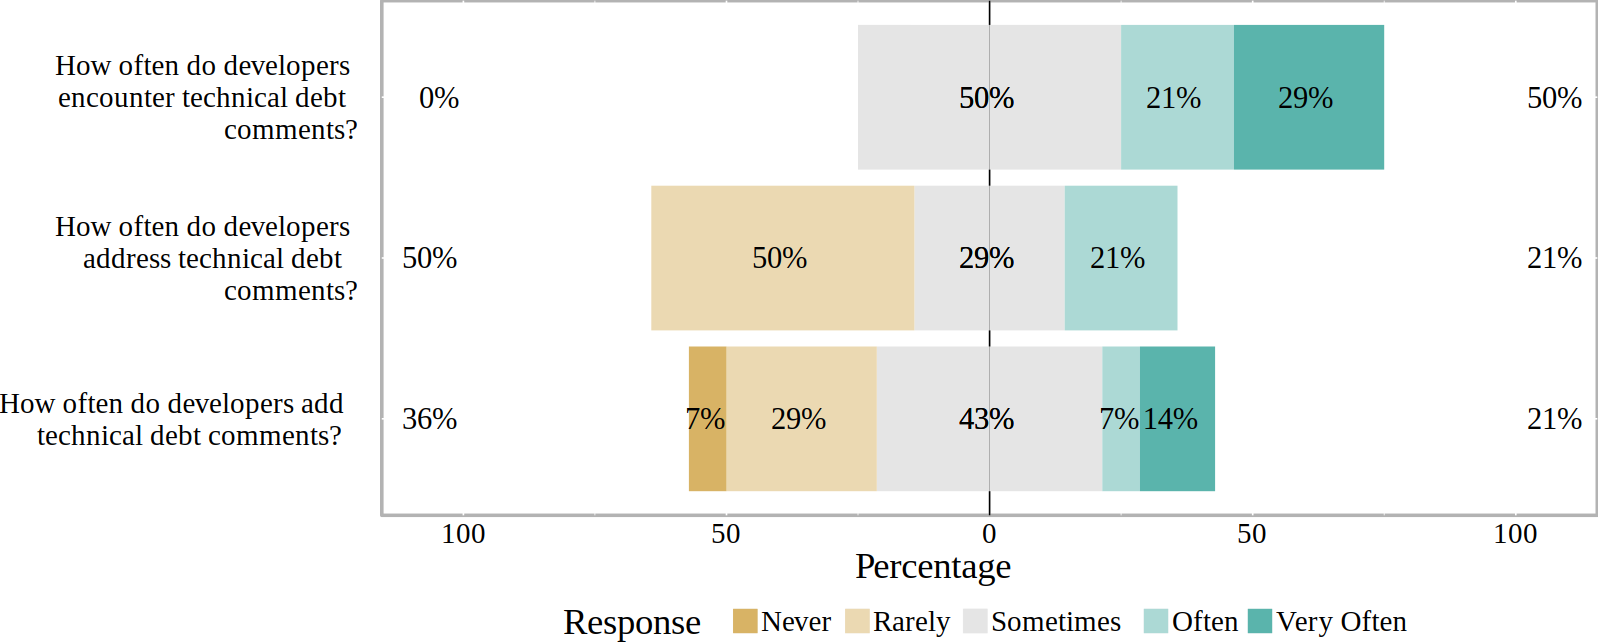
\includegraphics[width=0.95\columnwidth]{figures/test/_responses_question_.pdf}
 	\caption{Survey responses on how often do developers encounter, add, and address self-admitted technical debt.}
 	\label{fig:encouner_add_address}
 \end{figure}


As for why developers tend to add \SATD, nine respondents (P1, P4, P5, P8, P9, P11, P12, P13, and P14) indicated that they add self-admitted technical debt as \emph{a tracker in the source code for potential bugs or source code that needs to be improved or document a need for a new feature}. For example, P12 states that \textit{``It is usually a marker in the source of a missing feature or known bug.''}. Also, contrary to Postdar and Shihab~\cite{Potdar2014ICSME} we find that developers add self-admitted technical debt because of time pressure (P1, P2, P7, P13, and P14) to deliver tasks. For example, P1 said \textit{``Because they want to deliver, and when balancing an early delivery against technical debt."} Some other reasons for adding self-admitted technical debt are very rare and are only mentioned once or twice (e.g,. a remainder or looking for feedback). For example, P5 said that \textit{``They are not sure about the effects of their code and want feedback..."}.

In response to the question on why developers address self-admitted technical debt, we identified five reasons. The most cited reason for addressing self-admitted technical debt is \emph{to fix bugs} (P1, P4, P5, P7, P8, P9, P10, P12, and P13). For example, P12 states \textit{``, usually as part of fixing a user-reported issue..."} The second most frequent reasons is to add a new feature (P1, P4, P6, P12, and P14) and improve the code overall (P7, P8, P9, P10, and P11). The other two, less frequent, reasons are addressing \SATD when refactoring code (P7 and P9) and to provide a generally better solution (P2 and P7). Our findings indicate that there is a need for software projects to allocate resources to specifically address \SATD, since most respondents do not seem to indicate that there is a systematic process in place to address \SATD. And, in most cases it seems like dealing with \SATD is done in an ad-hoc manner.



 \conclusion{Developers add \SATD to track potential future bugs, code that needs improvements or areas to implement new features. Developers mostly remove \SATD when they are fixing bugs or adding new features. Very seldom do developers remove \SATD as part of refactoring efforts or dedicated code improvement activities.}
 

 
 
 